Circle $C_0$ has radius $1$, and the point $A_0$ is a point on the circle. Circle $C_1$ has radius $r<1$ and is internally tangent to $C_0$ at point $A_0$. Point $A_1$ lies on circle $C_1$ so that $A_1$ is located $90^{\circ}$ counterclockwise from $A_0$ on $C_1$. Circle $C_2$ has radius $r^2$ and is internally tangent to $C_1$ at point $A_1$. In this way a sequence of circles $C_1,C_2,C_3,...$ and a sequence of points on the circles $A_1,A_2,A_3,...$ are constructed, where circle $C_n$ has radius $r^n$ and is internally tangent to circle $C_{n-1}$ at point $A_{n-1}$, and point $A_n$ lies on $C_n$ $90^{\circ}$ counterclockwise from point $A_{n-1}$, as shown in the figure below. There is one point $B$ inside all of these circles. When $r=\frac{11}{60}$, the distance from the center of $C_0$ to $B$ is $\frac{m}{n}$, where $m$ and $n$ are relatively prime positive integers. Find $m+n$.

\begin{center}
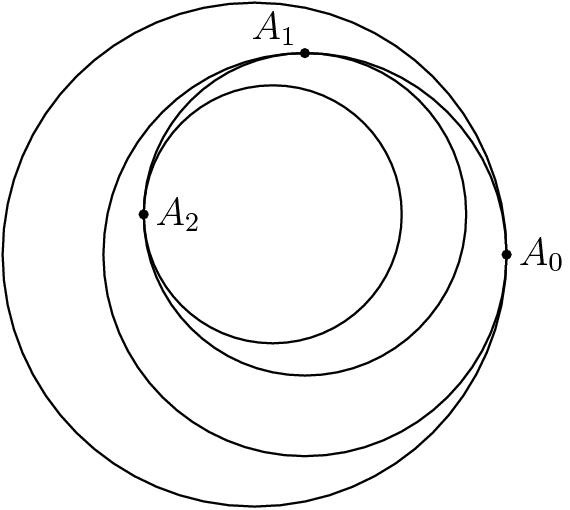
\includegraphics[width = 57.0mm]{img/fig0.png}
\end{center}